
\documentclass{standalone}
\usepackage{tikz}
\usetikzlibrary{arrows.meta,decorations.pathmorphing}

\begin{document}


\tikzset{every picture/.style={line width=0.75pt}} %set default line width to 0.75pt        

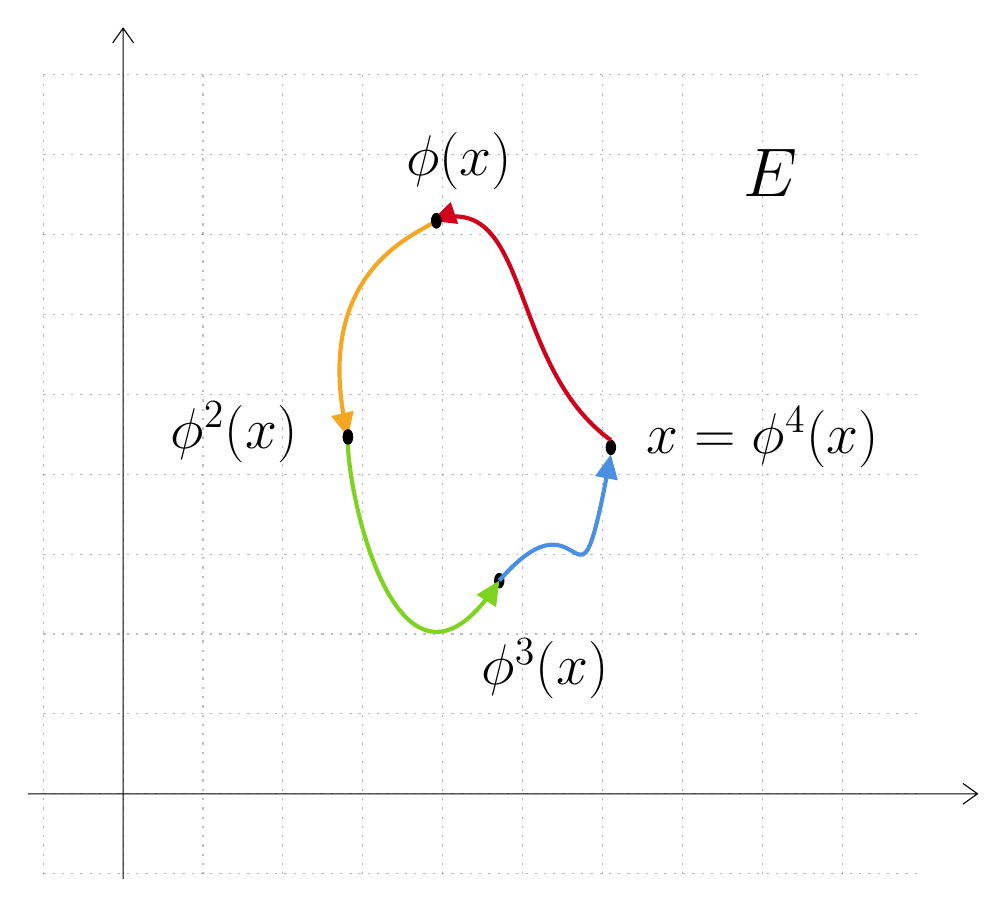
\begin{tikzpicture}[x=0.75pt,y=0.75pt,yscale=-1,xscale=1]
%uncomment if require: \path (0,446); %set diagram left start at 0, and has height of 446

%Shape: Axis 2D [id:dp5958965788842521] 
\draw  (26,374.85) -- (483.33,374.85)(71.73,6) -- (71.73,415.83) (476.33,369.85) -- (483.33,374.85) -- (476.33,379.85) (66.73,13) -- (71.73,6) -- (76.73,13)  ;
%Shape: Grid [id:dp4387530975228269] 
\draw  [draw opacity=0][dash pattern={on 0.84pt off 2.51pt}] (33.25,28.48) -- (456.59,28.48) -- (456.59,413.42) -- (33.25,413.42) -- cycle ; \draw  [color={rgb, 255:red, 0; green, 0; blue, 0 }  ,draw opacity=0.26 ][dash pattern={on 0.84pt off 2.51pt}] (33.25,28.48) -- (33.25,413.42)(71.73,28.48) -- (71.73,413.42)(110.22,28.48) -- (110.22,413.42)(148.7,28.48) -- (148.7,413.42)(187.19,28.48) -- (187.19,413.42)(225.67,28.48) -- (225.67,413.42)(264.16,28.48) -- (264.16,413.42)(302.64,28.48) -- (302.64,413.42)(341.13,28.48) -- (341.13,413.42)(379.62,28.48) -- (379.62,413.42)(418.1,28.48) -- (418.1,413.42) ; \draw  [color={rgb, 255:red, 0; green, 0; blue, 0 }  ,draw opacity=0.26 ][dash pattern={on 0.84pt off 2.51pt}] (33.25,28.48) -- (456.59,28.48)(33.25,66.97) -- (456.59,66.97)(33.25,105.45) -- (456.59,105.45)(33.25,143.94) -- (456.59,143.94)(33.25,182.42) -- (456.59,182.42)(33.25,220.91) -- (456.59,220.91)(33.25,259.39) -- (456.59,259.39)(33.25,297.88) -- (456.59,297.88)(33.25,336.36) -- (456.59,336.36)(33.25,374.85) -- (456.59,374.85)(33.25,413.34) -- (456.59,413.34) ; \draw  [color={rgb, 255:red, 0; green, 0; blue, 0 }  ,draw opacity=0.26 ][dash pattern={on 0.84pt off 2.51pt}]  ;
%Shape: Ellipse [id:dp45907299526679535] 
\draw  [fill={rgb, 255:red, 0; green, 0; blue, 0 }  ,fill opacity=1 ] (220.38,98.77) .. controls (220.38,96.86) and (221.38,95.31) .. (222.62,95.31) .. controls (223.86,95.31) and (224.87,96.86) .. (224.87,98.77) .. controls (224.87,100.67) and (223.86,102.22) .. (222.62,102.22) .. controls (221.38,102.22) and (220.38,100.67) .. (220.38,98.77) -- cycle ;
%Shape: Ellipse [id:dp8007635814883884] 
\draw  [fill={rgb, 255:red, 0; green, 0; blue, 0 }  ,fill opacity=1 ] (250.71,272.15) .. controls (250.71,270.24) and (251.71,268.69) .. (252.95,268.69) .. controls (254.19,268.69) and (255.19,270.24) .. (255.19,272.15) .. controls (255.19,274.05) and (254.19,275.6) .. (252.95,275.6) .. controls (251.71,275.6) and (250.71,274.05) .. (250.71,272.15) -- cycle ;
%Shape: Ellipse [id:dp42119274412116026] 
\draw  [fill={rgb, 255:red, 0; green, 0; blue, 0 }  ,fill opacity=1 ] (304.47,207.94) .. controls (304.47,206.03) and (305.47,204.49) .. (306.71,204.49) .. controls (307.95,204.49) and (308.96,206.03) .. (308.96,207.94) .. controls (308.96,209.85) and (307.95,211.39) .. (306.71,211.39) .. controls (305.47,211.39) and (304.47,209.85) .. (304.47,207.94) -- cycle ;
%Shape: Ellipse [id:dp8208200284508345] 
\draw  [fill={rgb, 255:red, 0; green, 0; blue, 0 }  ,fill opacity=1 ] (177.78,202.9) .. controls (177.78,201) and (178.79,199.45) .. (180.03,199.45) .. controls (181.27,199.45) and (182.27,201) .. (182.27,202.9) .. controls (182.27,204.81) and (181.27,206.36) .. (180.03,206.36) .. controls (178.79,206.36) and (177.78,204.81) .. (177.78,202.9) -- cycle ;
%Curve Lines [id:da6003053339078104] 
\draw [color={rgb, 255:red, 208; green, 2; blue, 27 }  ,draw opacity=1 ][line width=1.5]    (306.71,204.49) .. controls (257.32,168.75) and (268.2,86.48) .. (223.9,97.72) ;
\draw [shift={(220.38,98.77)}, rotate = 341.15] [fill={rgb, 255:red, 208; green, 2; blue, 27 }  ,fill opacity=1 ][line width=0.08]  [draw opacity=0] (11.61,-5.58) -- (0,0) -- (11.61,5.58) -- cycle    ;
%Curve Lines [id:da20886796664244178] 
\draw [color={rgb, 255:red, 245; green, 166; blue, 35 }  ,draw opacity=1 ][line width=1.5]    (222.62,98.77) .. controls (214.31,104.98) and (162.62,121.97) .. (179.22,199.33) ;
\draw [shift={(180.03,202.9)}, rotate = 256.71] [fill={rgb, 255:red, 245; green, 166; blue, 35 }  ,fill opacity=1 ][line width=0.08]  [draw opacity=0] (11.61,-5.58) -- (0,0) -- (11.61,5.58) -- cycle    ;
%Curve Lines [id:da2996907087164338] 
\draw [color={rgb, 255:red, 126; green, 211; blue, 33 }  ,draw opacity=1 ][line width=1.5]    (180.03,202.9) .. controls (178.82,228.31) and (203.95,344.01) .. (250.79,275.41) ;
\draw [shift={(252.95,272.15)}, rotate = 122.6] [fill={rgb, 255:red, 126; green, 211; blue, 33 }  ,fill opacity=1 ][line width=0.08]  [draw opacity=0] (11.61,-5.58) -- (0,0) -- (11.61,5.58) -- cycle    ;
%Shape: Ellipse [id:dp47532939931231355] 
\draw  [fill={rgb, 255:red, 0; green, 0; blue, 0 }  ,fill opacity=1 ] (220.38,98.77) .. controls (220.38,96.86) and (221.38,95.31) .. (222.62,95.31) .. controls (223.86,95.31) and (224.87,96.86) .. (224.87,98.77) .. controls (224.87,100.67) and (223.86,102.22) .. (222.62,102.22) .. controls (221.38,102.22) and (220.38,100.67) .. (220.38,98.77) -- cycle ;
%Shape: Ellipse [id:dp2599959930388829] 
\draw  [fill={rgb, 255:red, 0; green, 0; blue, 0 }  ,fill opacity=1 ] (177.78,202.9) .. controls (177.78,201) and (178.79,199.45) .. (180.03,199.45) .. controls (181.27,199.45) and (182.27,201) .. (182.27,202.9) .. controls (182.27,204.81) and (181.27,206.36) .. (180.03,206.36) .. controls (178.79,206.36) and (177.78,204.81) .. (177.78,202.9) -- cycle ;
%Curve Lines [id:da849505314209388] 
\draw [color={rgb, 255:red, 74; green, 144; blue, 226 }  ,draw opacity=1 ][line width=1.5]    (252.95,272.15) .. controls (296.2,222.26) and (288.97,305.55) .. (306.18,214.22) ;
\draw [shift={(306.71,211.39)}, rotate = 100.58] [fill={rgb, 255:red, 74; green, 144; blue, 226 }  ,fill opacity=1 ][line width=0.08]  [draw opacity=0] (11.61,-5.58) -- (0,0) -- (11.61,5.58) -- cycle    ;

% Text Node
\draw (369.58,62.93) node [anchor=north west][inner sep=0.75pt]  [font=\Huge]  {$E$};
% Text Node
\draw (206.84,55.02) node [anchor=north west][inner sep=0.75pt]  [font=\huge]  {$\phi ( x)$};
% Text Node
\draw (93.38,184.95) node [anchor=north west][inner sep=0.75pt]  [font=\huge]  {$\phi ^{2}( x)$};
% Text Node
\draw (243.18,298.73) node [anchor=north west][inner sep=0.75pt]  [font=\huge]  {$\phi ^{3}( x)$};
% Text Node
\draw (322.75,187.33) node [anchor=north west][inner sep=0.75pt]  [font=\huge]  {$x=\phi ^{4}( x)$};


\end{tikzpicture}

\end{document}